\documentclass{article}
\usepackage{cite}
\usepackage{amsmath,amssymb,amsfonts}
\usepackage{graphicx}
\newtheorem{theorem}{Theorem}
\newtheorem{lemma}{Lemma}
\newtheorem{definition}{Definition}
\newtheorem{note}{Note}
\newtheorem{property}{Property}

\newcommand{\fbf}{\mathbf{f}}
\newcommand{\Jbf}{\mathbf{J}}
\newcommand{\Mbf}{\mathbf{M}}
\newcommand{\mbf}{\mathbf{m}}
\newcommand{\pbf}{\mathbf{p}}
\newcommand{\ubf}{\mathbf{u}}
\newcommand{\vbf}{\mathbf{v}}
\newcommand{\deltabf}{\boldsymbol{\delta}}
\newcommand{\omegabf}{\boldsymbol{\omega}}
\newcommand{\taubf}{\boldsymbol{\tau}}


\title{Path Planning Challenge}
\author{Magicc Lab, Summer 2023}
\date{\today}

\begin{document}

\maketitle
\thispagestyle{empty}

    \begin{abstract}
        Convex optimization challenge for summer 2023.
    \end{abstract}

%-------------------------------------------------------
\section{Introduction}

The convex optimization challenge will use the VTOL example from~\cite{BeardMcLainPeterson}, which is describe below for convenience.  


\begin{figure}
  % Requires \usepackage{graphicx}
  \centering
  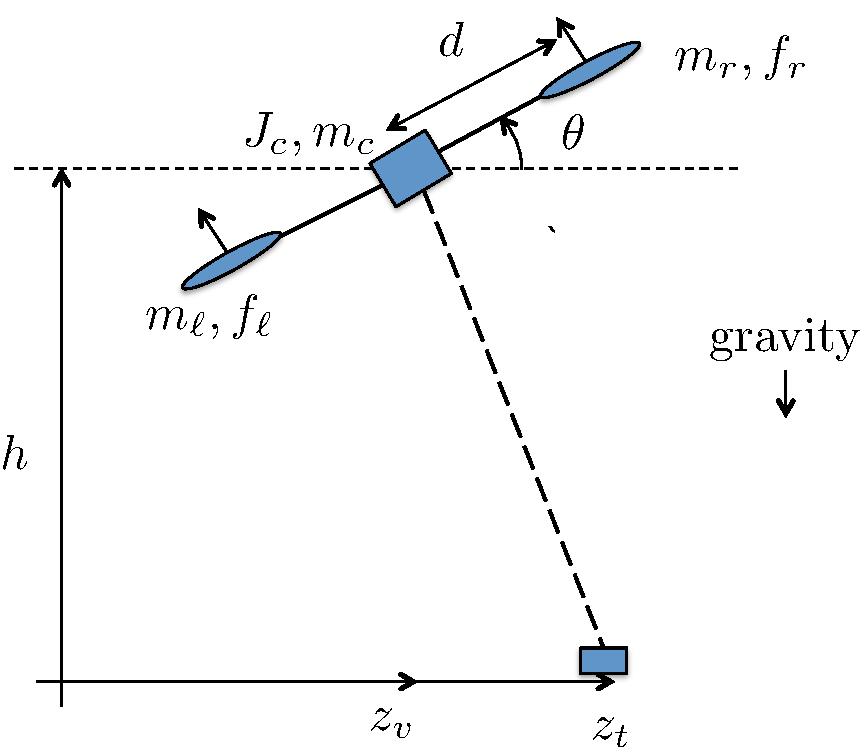
\includegraphics[width=0.59\textwidth]{figures/hw_planar_VTOL_defn}\\
  \caption{Planar vertical take-off and landing (VTOL)}
  \label{fig:planar_VTOL_defn}
\end{figure}

In this design study we will explore the control design for a simplified planar version of a quadrotor following a ground target.  In particular, we will constrain the dynamics to be in two a dimensional plane. In Cartesian space, the position of the VTOL can be defined by a variable describing the vertical position, one describing the horizontal position, and one angular variable describing the orientation, as shown in \ref{fig:planar_VTOL_defn}.  The planar vertical take-off and landing (VTOL) system is comprised of a center pod of mass $m_c$ and inertia $J_c$, a right motor/rotor that is modeled as a point mass $m_r$ that exerts a force $f_r$ at a distance $d$ from the center of mass, and a left motor/rotor that is modeled as a point mass $m_\ell$ that exerts a force $f_\ell$ at a distance $-d$ from the center of mass.  The position of the center of mass of the planar VTOL system is given by horizontal position $z_v$ and altitude $h$.  The airflow through the rotor creates a change in the direction of flow of air and causes what is called ``momentum drag.''  Momentum drag can be modeled as a viscous drag force that is proportional to the horizontal velocity $\dot{z}_v$.  In other words, the drag force is $F_{\text{drag}}=-\mu \dot{z}_v$.  The target on the ground will be modeled as an object with position $z_t$ and altitude $h=0$.  We will not explicitly model the dynamics of the target.  

Use the following physical parameters:
$m_c=1$~kg,
$J_c=0.0042$~kg m$^2$,
$m_r=0.25$~kg,
$m_\ell=0.25$~kg,
$d=0.3$~m,
$\mu = 0.1$~kg/s,
$g=9.81$~m/s$^2$.





%-------------------------------------------------------
\section{Dynamics}

The dynamics are given by
\begin{equation}\label{eq:vtol_sim_model}
\begin{pmatrix}
m_c + 2 m_r & 0           & 0 \\
0           & m_c + 2 m_r & 0 \\
0           & 0           & J_c + 2 m_r d^2
\end{pmatrix}
\begin{pmatrix}
\ddot{z} \\
\ddot{h} \\
\ddot{\theta}
\end{pmatrix}
=
\begin{pmatrix}
-(f_r + f_\ell) \sin\theta - \mu\dot{z} \\
-(m_c + 2 m_r) g + (f_r + f_\ell) \cos\theta \\
d \left( f_r - f_\ell \right)
\end{pmatrix}.
\end{equation}

We will assume that the right and left rotor forces are constrained as follows
\begin{equation}\label{eq:input_constraints}
	0\leq f_r, f_\ell \leq 0.75 (m_c + 2 m_r)g.
\end{equation}
If the thrust was limited to $0.5 (m_c + 2 m_r)g$, then at full throttle, the VTOL could just hover.  Therefore, the limit allows some additional control authority, but is somewhat constraining.

%-------------------------------------------------------
\section{Trajectory Following}

We will assume that a state-space controller with integrator is designed for the system as described in Chapter~12 of~\cite{BeardMcLainPeterson}, and that a disturbance observer is used to estimate the states as described in Chapter~14 of~\cite{BeardMcLainPeterson}.  The input to the system is the desired forward position $z^r(t)$ and the desired altitude $h^r(t)$.  


\bibliographystyle{IEEEtran}
\bibliography{library}

\end{document}

